\documentclass{article}
\usepackage[utf8]{inputenc}
\usepackage[spanish]{babel}
\usepackage{listings}
\usepackage{graphicx}
\graphicspath{ {images/} }
\usepackage{cite}

\begin{document}

\begin{titlepage}
    \begin{center}
        \vspace*{1cm}
            
        \Huge
        \textbf{Informa2 S.A.S}
            
        \vspace{0.5cm}
        \LARGE
        Parcial 2
            
        \vspace{1.5cm}
            
        \textbf{Carolina Jimenez Restrepo}
            
        \vfill
            
        \vspace{0.8cm}
            
        \Large
        Despartamento de Ingeniería Electrónica y Telecomunicaciones\\
        Universidad de Antioquia\\
        Medellín\\
        Septiembre de 2021
            
    \end{center}
\end{titlepage}

\tableofcontents
\newpage
\section{Sección introductoria}\label{intro}
Análisis y diseño del segundo parcial, presentar una imagen en matriz de LEDs RGB 



\section{Inclusión de imágenes} \label{imagenes}

En la Figura (\ref{fig:Matriz leds.png}), se presenta la matriz de LEDs con la que se trabajara, esta matriz esta dispuesta a cambios segun lo requiera el avance del desafio 

\begin{figure}[h]
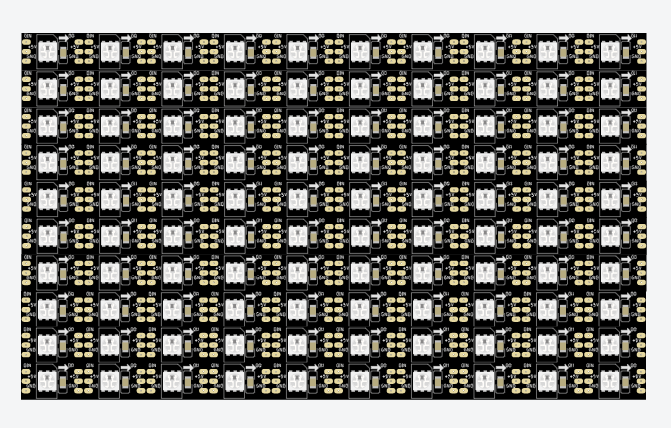
\includegraphics[width=4cm]{Matriz leds.png}
\centering
\caption{Matriz LEDs RGB}
\label{fig:Matriz leds.png}
\end{figure}


\end{document}
